% Options for packages loaded elsewhere
\PassOptionsToPackage{unicode}{hyperref}
\PassOptionsToPackage{hyphens}{url}
%
\documentclass[
  a4paper]{article}
\usepackage{amsmath,amssymb}
\usepackage{iftex}
\ifPDFTeX
  \usepackage[T1]{fontenc}
  \usepackage[utf8]{inputenc}
  \usepackage{textcomp} % provide euro and other symbols
\else % if luatex or xetex
  \usepackage{unicode-math} % this also loads fontspec
  \defaultfontfeatures{Scale=MatchLowercase}
  \defaultfontfeatures[\rmfamily]{Ligatures=TeX,Scale=1}
\fi
\usepackage{lmodern}
\ifPDFTeX\else
  % xetex/luatex font selection
\fi
% Use upquote if available, for straight quotes in verbatim environments
\IfFileExists{upquote.sty}{\usepackage{upquote}}{}
\IfFileExists{microtype.sty}{% use microtype if available
  \usepackage[]{microtype}
  \UseMicrotypeSet[protrusion]{basicmath} % disable protrusion for tt fonts
}{}
\makeatletter
\@ifundefined{KOMAClassName}{% if non-KOMA class
  \IfFileExists{parskip.sty}{%
    \usepackage{parskip}
  }{% else
    \setlength{\parindent}{0pt}
    \setlength{\parskip}{6pt plus 2pt minus 1pt}}
}{% if KOMA class
  \KOMAoptions{parskip=half}}
\makeatother
\usepackage{xcolor}
\usepackage[margin=1in]{geometry}
\usepackage{longtable,booktabs,array}
\usepackage{calc} % for calculating minipage widths
% Correct order of tables after \paragraph or \subparagraph
\usepackage{etoolbox}
\makeatletter
\patchcmd\longtable{\par}{\if@noskipsec\mbox{}\fi\par}{}{}
\makeatother
% Allow footnotes in longtable head/foot
\IfFileExists{footnotehyper.sty}{\usepackage{footnotehyper}}{\usepackage{footnote}}
\makesavenoteenv{longtable}
\usepackage{graphicx}
\makeatletter
\def\maxwidth{\ifdim\Gin@nat@width>\linewidth\linewidth\else\Gin@nat@width\fi}
\def\maxheight{\ifdim\Gin@nat@height>\textheight\textheight\else\Gin@nat@height\fi}
\makeatother
% Scale images if necessary, so that they will not overflow the page
% margins by default, and it is still possible to overwrite the defaults
% using explicit options in \includegraphics[width, height, ...]{}
\setkeys{Gin}{width=\maxwidth,height=\maxheight,keepaspectratio}
% Set default figure placement to htbp
\makeatletter
\def\fps@figure{htbp}
\makeatother
\setlength{\emergencystretch}{3em} % prevent overfull lines
\providecommand{\tightlist}{%
  \setlength{\itemsep}{0pt}\setlength{\parskip}{0pt}}
\setcounter{secnumdepth}{-\maxdimen} % remove section numbering
\usepackage{float} \usepackage{multirow}
\ifLuaTeX
  \usepackage{selnolig}  % disable illegal ligatures
\fi
\usepackage{bookmark}
\IfFileExists{xurl.sty}{\usepackage{xurl}}{} % add URL line breaks if available
\urlstyle{same}
\hypersetup{
  hidelinks,
  pdfcreator={LaTeX via pandoc}}

\author{}
\date{\vspace{-2.5em}}

\begin{document}

\section{Question 1}\label{question-1}

\begin{enumerate}
\def\labelenumi{\roman{enumi})}
\item
  Name the three basic principles in experimental design.
\item
  Why is replication important in experimental design?
\item
  What is the main purpose for using randomization in an experiment?
\end{enumerate}

Water flow velocities have been suspected to affect the growth of fish
species like California halibut (\emph{Paralichthys californicus}). The
California halibut (\emph{Paralichthys californicus}) is an economically
important flatfish species of Southern California in the USA. A study
was carried out to test the effect of three relative water velocities of
0.5, 1.0, and 1.5 on the gain of bodyweight of California halibut over a
period of 10 weeks. Nine rectangular tanks filled with fifteen (15)
California halibut fish each were given to set the velocities to be
tested. All the fish were of the same age, same weight, and same health
status. Furthermore, all fish were fed the same food. All experimental
tanks are the same in length, width, and depth. All tanks receive the
same environmental conditions. Three experimental tanks were randomly
assigned to each velocity. The experiment was fully randomized. After 10
weeks, the body weight of each fish was measured. Each fish was
individually weighted and immediately returned to its respective
experimental tank.~

\begin{enumerate}
\def\labelenumi{\roman{enumi})}
\setcounter{enumi}{3}
\item
  Write the following with reference to this experiment.

  \begin{enumerate}
  \def\labelenumii{(\alph{enumii})}
  \item
    Experimental unit
  \item
    Observation unit
  \item
    Factor/ Factors tested
  \item
    Factor levels
  \item
    Treatments tested
  \item
    Response variable
  \item
    How many replicates are there for each treatment?
  \end{enumerate}
\item
  If you do this experiment, how would you employ randomization?
\item
  Write the most suitable statistical model for the experiment. Define
  all terms in it and state any assumptions you make regarding the
  model.
\end{enumerate}

\section{Question 2}\label{question-2}

An experiment was performed to determine the effect of four different
chemicals on the strength of a fabric. These chemicals are used as part
of the design printing process. Five different fabric samples were
selected. The experiment was carried out by testing each chemical type
on each fabric sample once in a random order. The data is shown in the
table below.

\begin{table}[!h]
\centering
\caption{Question 2 data}
\begin{tabular}{|l|lllll|}
\hline
\multirow{2}{*}{Chemical Type} & \multicolumn{5}{l|}{Fabric Sample}                                                                            \\ \cline{2-6} 
                 & \multicolumn{1}{l|}{1} & \multicolumn{1}{l|}{2} & \multicolumn{1}{l|}{3} & \multicolumn{1}{l|}{4} &  5 \\ \hline
            A      &  \multicolumn{1}{l|}{24} & \multicolumn{1}{l|}{23} & \multicolumn{1}{l|}{26} & \multicolumn{1}{l|}{28} & 22 \\ \hline
             B     & \multicolumn{1}{l|}{32} & \multicolumn{1}{l|}{33} & \multicolumn{1}{l|}{24} & \multicolumn{1}{l|}{36} & 28 \\ \hline
             C     & \multicolumn{1}{l|}{34} & \multicolumn{1}{l|}{33} & \multicolumn{1}{l|}{29} & \multicolumn{1}{l|}{37} & 37 \\ \hline
              D    & \multicolumn{1}{l|}{40} & \multicolumn{1}{l|}{32} & \multicolumn{1}{l|}{33} & \multicolumn{1}{l|}{41} & 37 \\ \hline
\end{tabular}
\end{table}

These data were given to two students separately and asked to construct
the ANOVA table to analyze. The results obtained by them are given
below. Some values were missing in each ANOVA table and marked with a
blank space (\ldots).

\begin{enumerate}
\def\labelenumi{\roman{enumi})}
\tightlist
\item
  Complete each ANOVA table below (Copy the tables below in your answer
  script and complete it.)
\end{enumerate}

\emph{Results of the first student}

\begin{longtable}[]{@{}llllll@{}}
\toprule\noalign{}
Source & DF & SS & MS & F & P \\
\midrule\noalign{}
\endhead
\bottomrule\noalign{}
\endlastfoot
Chemical type & \ldots{} & \ldots{} & \ldots{} & \ldots{} & 0.000 \\
Error & \ldots{} & 219.6 & \ldots{} & & \\
Total & \ldots{} & 623 & & & \\
\end{longtable}

\emph{Results of the second student}

\begin{longtable}[]{@{}llllll@{}}
\toprule\noalign{}
Source & DF & SS & MS & F & P \\
\midrule\noalign{}
\endhead
\bottomrule\noalign{}
\endlastfoot
Chemical type & \ldots{} & \ldots{} & \ldots{} & \ldots{} & 0.000 \\
Fabric sample & \ldots{} & 124.2 & \ldots{} & \ldots{} & 0.029 \\
Error & \ldots{} & 95.4 & \ldots{} & & \\
Total & \ldots{} & 623 & & & \\
\end{longtable}

\begin{enumerate}
\def\labelenumi{\roman{enumi})}
\setcounter{enumi}{1}
\item
  State the differences between the two approaches the two students had
  applied.
\item
  One student has obtained the following graph. Comment on it.
\end{enumerate}

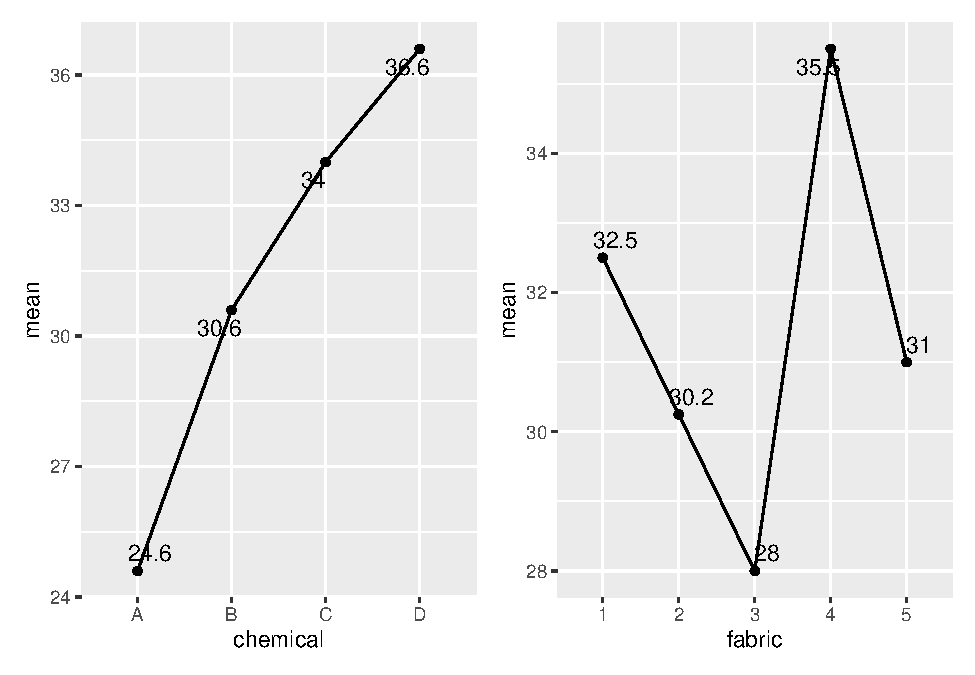
\includegraphics{index_files/figure-latex/unnamed-chunk-4-1.pdf}

\begin{enumerate}
\def\labelenumi{\roman{enumi})}
\setcounter{enumi}{3}
\item
  What is the best approach (first student approach or second student
  approach)? Justify your answer.
\item
  Write the effect model for the selected approach in part (iv) and
  define all the terms of it.
\item
  Write the hypothesis of the selected model to test the equality of
  treatment means and state your decision and conclusion. (No need to do
  multiple comparisons.)
\end{enumerate}

\section{Question 3}\label{question-3}

Twenty four (24) pieces of metal pipes were chosen for an experiment to
examine if the quantity of corrosion is affected by the coating type or
the soil type. The experiment uses two different coating types and three
different soil types. Each metal item is coated with one of the two
coatings and buried for a specific amount of time in one of the three
types of soil, after which the quantity of corrosion is calculated. The
data obtained is presented in the table below.

\begin{table}[!h]
\centering
\begin{tabular}{|l|llll|}
\hline
\multirow{2}{*}{Soil type} & \multicolumn{4}{l|}{Coating type}                                                    \\ \cline{2-5} 
                  & \multicolumn{2}{l|}{1}                         & \multicolumn{2}{l|}{2}    \\ \hline
\multirow{2}{*}{1} & \multicolumn{1}{l|}{7} & \multicolumn{1}{l|}{8} & \multicolumn{1}{l|}{10} & 15 \\ \cline{2-5} 
                  & \multicolumn{1}{l|}{14} & \multicolumn{1}{l|}{9} & \multicolumn{1}{l|}{11} & 6 \\ \hline
\multirow{2}{*}{2} & \multicolumn{1}{l|}{11} & \multicolumn{1}{l|}{12} & \multicolumn{1}{l|}{16} & 15 \\ \cline{2-5} 
                  & \multicolumn{1}{l|}{17} & \multicolumn{1}{l|}{14} & \multicolumn{1}{l|}{13} & 20 \\ \hline
\multirow{2}{*}{3} & \multicolumn{1}{l|}{11} & \multicolumn{1}{l|}{4} & \multicolumn{1}{l|}{17} & 19 \\ \cline{2-5} 
                  & \multicolumn{1}{l|}{12} & \multicolumn{1}{l|}{9} & \multicolumn{1}{l|}{17} & 18 \\ \hline
\end{tabular}
\end{table}

\begin{enumerate}
\def\labelenumi{\roman{enumi})}
\item
  How many treatment combinations are tested in this experiment? What
  are they?
\item
  The mean plot of the above data is given below. Comment on it.
\end{enumerate}

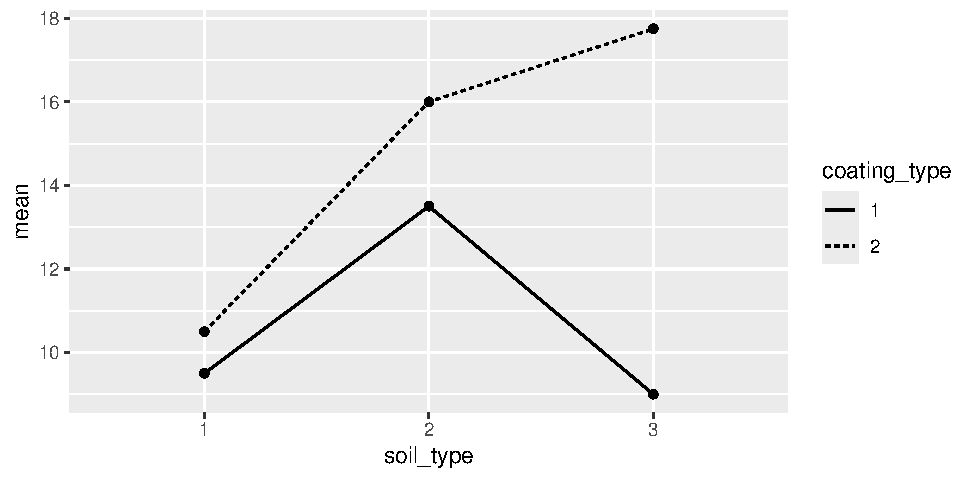
\includegraphics{index_files/figure-latex/unnamed-chunk-6-1.pdf}

\begin{enumerate}
\def\labelenumi{\roman{enumi})}
\setcounter{enumi}{2}
\item
  Write a suitable effect model for the experiment and state the
  hypotheses to be tested.
\item
  ANOVA table for the above experiment is given below. State your
  conclusions. Assume that the assumptions of the model are not
  violated.
\end{enumerate}

\begin{verbatim}
Analysis of Variance Table

Response: corrosion_amount
                       Df  Sum Sq Mean Sq F value   Pr(>F)   
soil_type               2  95.583  47.792  5.4532 0.014076 * 
coating_type            1 100.042 100.042 11.4152 0.003346 **
soil_type:coating_type  2  67.583  33.792  3.8558 0.040392 * 
Residuals              18 157.750   8.764                    
---
Signif. codes:  0 '***' 0.001 '**' 0.01 '*' 0.05 '.' 0.1 ' ' 1
\end{verbatim}

\begin{enumerate}
\def\labelenumi{\alph{enumi})}
\setcounter{enumi}{21}
\tightlist
\item
  For further investigation, the Tukey multiple comparison tests were
  performed. The results are given below. Comment on the results and
  what should you recommend to reduce the amount of corrosion (give
  reasons for your answer)?
\end{enumerate}

\begin{verbatim}
  Tukey multiple comparisons of means
    95% family-wise confidence level

Fit: aov(formula = corrosion_amount ~ soil_type * coating_type, data = q3)

$soil_type
      diff        lwr      upr     p adj
2-1  4.750  0.9723052 8.527695 0.0128436
3-1  3.375 -0.4026948 7.152695 0.0846412
3-2 -1.375 -5.1526948 2.402695 0.6295541

$coating_type
        diff      lwr     upr     p adj
2-1 4.083333 1.544216 6.62245 0.0033461

$`soil_type:coating_type`
         diff         lwr       upr     p adj
2:1-1:1  4.00  -2.6526105 10.652611 0.4272548
3:1-1:1 -0.50  -7.1526105  6.152611 0.9998730
1:2-1:1  1.00  -5.6526105  7.652611 0.9963915
2:2-1:1  6.50  -0.1526105 13.152611 0.0577047
3:2-1:1  8.25   1.5973895 14.902611 0.0104439
3:1-2:1 -4.50 -11.1526105  2.152611 0.3071941
1:2-2:1 -3.00  -9.6526105  3.652611 0.7076774
2:2-2:1  2.50  -4.1526105  9.152611 0.8338901
3:2-2:1  4.25  -2.4026105 10.902611 0.3643703
1:2-3:1  1.50  -5.1526105  8.152611 0.9773677
2:2-3:1  7.00   0.3473895 13.652611 0.0358934
3:2-3:1  8.75   2.0973895 15.402611 0.0063084
2:2-1:2  5.50  -1.1526105 12.152611 0.1409369
3:2-1:2  7.25   0.5973895 13.902611 0.0281668
3:2-2:2  1.75  -4.9026105  8.402611 0.9566132
\end{verbatim}

\section{Question 4}\label{question-4}

A materials science engineer is investigating the effects of four
different catalysts (A, B, C, and D) on the reaction time of a chemical
process. Each batch of new material is only large enough to permit four
runs to be made. Furthermore, four lab assistants were selected for the
study. To account for the source of variability due to batch and lab
assistant, the engineer uses the Latin square design shown below.

\begin{table}[!h]
\centering
\begin{tabular}{|l|llll|}
\hline
\multirow{2}{*}{Batch} & \multicolumn{4}{l|}{Lab assistant}                                                    \\ \cline{2-5} 
                  & \multicolumn{1}{l|}{1} & \multicolumn{1}{l|}{2} & \multicolumn{1}{l|}{3} & 4 \\ \hline
                 1 & \multicolumn{1}{l|}{C=8} & \multicolumn{1}{l|}{D=7} & \multicolumn{1}{l|}{A=1} &  B=6\\ \hline
               2   & \multicolumn{1}{l|}{B=11} & \multicolumn{1}{l|}{C=18} & \multicolumn{1}{l|}{D=11} & A=9 \\ \hline
               3   & \multicolumn{1}{l|}{A=5} & \multicolumn{1}{l|}{B=8} & \multicolumn{1}{l|}{C=10} & D=9 \\ \hline
                4  & \multicolumn{1}{l|}{D=4} & \multicolumn{1}{l|}{A=3} & \multicolumn{1}{l|}{B=5} & C=6 \\ \hline
\end{tabular}
\end{table}

\begin{enumerate}
\def\labelenumi{\roman{enumi})}
\tightlist
\item
  Is this a standard Latin square design? Give reasons for your answer.
\end{enumerate}

Cont. page 6

\newpage

\begin{enumerate}
\def\labelenumi{\roman{enumi})}
\setcounter{enumi}{1}
\tightlist
\item
  ANOVA table for the above experiment is given below. Write the model
  corresponding to the ANOVA. Define all terms in it. State any
  assumptions you make regarding the model.
\end{enumerate}

\begin{verbatim}
Analysis of Variance Table

Response: Time
              Df  Sum Sq Mean Sq F value    Pr(>F)    
Batch          3 143.187  47.729 27.6024 0.0006573 ***
Lab_assistant  3  12.188   4.063  2.3494 0.1717719    
Catalyst       3  72.188  24.063 13.9157 0.0041308 ** 
Residuals      6  10.375   1.729                      
---
Signif. codes:  0 '***' 0.001 '**' 0.01 '*' 0.05 '.' 0.1 ' ' 1
\end{verbatim}

\begin{enumerate}
\def\labelenumi{\roman{enumi})}
\setcounter{enumi}{2}
\item
  Briefly explain how you check the validity of the model assumptions.
\item
  Assume that the estimated model in part (ii) satisfied all of the
  assumptions made regarding the error term. What conclusions can be
  drawn from the results of ANOVA table. You should clearly write the
  corresponding hypotheses, decision and conclusions.
\item
  Write one advantage and one disadvantage of a Latin square design.
\end{enumerate}

\end{document}
